%\providecommand{\main}{..}
%\documentclass[\main/main.tex]{subfiles}


\begin{document}

\section{Computing Mortality}

In order to set up our model, we need the mortality rates by age group. \cite{Caswell2018} suggest using the Human Mortality Database (HMD), which is one of the most renowned sources to study longevity of our times.
The database contains both period and cohort life tables (by country or area) and provides information starting from the 19th, 20th, or mid-20th century, depending on the census coverage of the country. \\

One major disadvantage for our analysis, though, is that the HMD provides mortality rates aggregating all causes of death. Conversely, we need mortality data by status, i.e. for healthy and disabled individuals separately. Indeed, if we were to apply the same mortality regime to all individuals, we would be assuming that having a disability does not have an effect on the probability of dying. This does not seem reasonable since by \lq\lq being disabled'' we mean \lq\lq not being able to perform any of the following task: dressing, bathing or showering, eating and cutting up food, walking across a room, and getting in or out of bed''. The above conditions are likely to be the result of poor health and this increased vulnerability of individuals may in turn increase their risk of death.\\

As a second possibility, we explored the data provided by the Global Burden of Diseases (GBD). 
This dataset provides a information about premature death and disability and identifies more than 300 diseases and injuries as possible causes of death. However, despite the broad spectrum of risk factors considered, also the GBD does not provide data of disability as it defined in this study.\\

Therefore, we eventually decided to estimate mortality data directly from SHARE and compare our estimates to the information contained in the life tables of the HMD. This should give us and indication on whether we are overestimating/underestimating the mortality regime for our population.



\subsection{Estimates of mortality probability from SHARE}




\subsection{Estimates of mortality probability from HMD}

We are going to construct an average of the probability of death from the HMD that should at best compare to the estimates from SHARE. The method we followed is briefly outlined below.\\

First of all, we downloaded from the HMD website the period life tables for our nine selected countries. A period life table represents the hypothetical experience of a synthetic cohort, i.e. a cohort that follows the age-specific death rates of a given period. These rates can be computed by looking at the mortality experience of all cohorts who are present during the period and then by \lq\lq hypothetically'' applying them to the synthetic cohort.\\
In other words, the life tables from the HMD describe the distribution of the time it takes the synthetic cohort of individuals to experience the \lq\lq death'' event. The HMD describes this distribution for each separate year. In particular, we are considering the value of
$q_x$ in the life table, i.e. the probability of dying between (exact) age $x$ and (exact) age $x+1$. \\

As a second step, we selected only those years corresponding to the years of interviews in SHARE, namely 2004, 2005,  2006, 2007,2009, 2010, 2011, 2012, 2013. Figure \ref{dying_female} and \ref{dying_male} show the probability of dying from one year to the next, starting from age 50 up to age 90, for female and male population respectively, as retrieved from the HMD life tables. As expected, the mortality risk has not changed much over the ten-year time horizon we are considering.


\begin{figure}[H]
\centering \textbf{Female population}\par\medskip
\minipage{0.32\textwidth}
  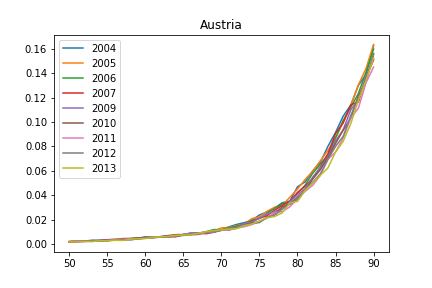
\includegraphics[width=\linewidth]{images/mortality_female_1.png}
\endminipage\hfill
\minipage{0.32\textwidth}
  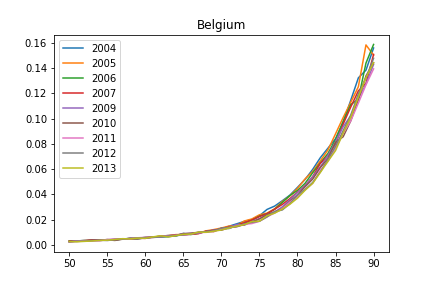
\includegraphics[width=\linewidth]{images/mortality_female_2.png}
\endminipage\hfill
\minipage{0.32\textwidth}%
  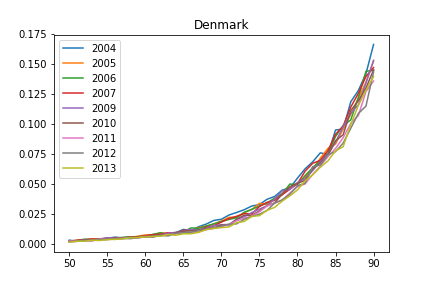
\includegraphics[width=\linewidth]{images/mortality_female_3.png}
\endminipage \hfill
\minipage{0.32\textwidth}
  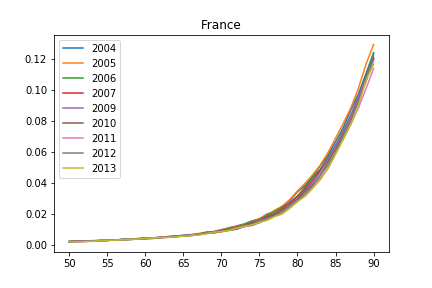
\includegraphics[width=\linewidth]{images/mortality_female_4.png}
\endminipage\hfill
\minipage{0.32\textwidth}
  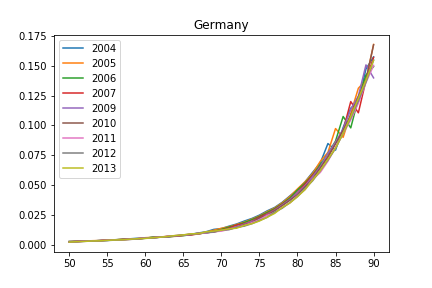
\includegraphics[width=\linewidth]{images/mortality_female_5.png}
\endminipage\hfill
\minipage{0.32\textwidth}%
  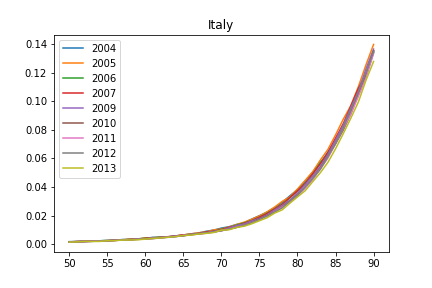
\includegraphics[width=\linewidth]{images/mortality_female_6.png}
\endminipage\hfill
\minipage{0.32\textwidth}
  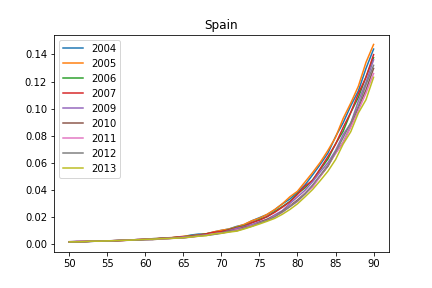
\includegraphics[width=\linewidth]{images/mortality_female_7.png}
\endminipage\hfill
\minipage{0.32\textwidth}
  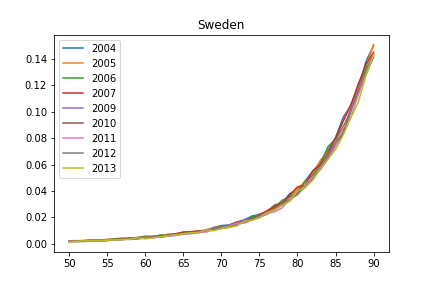
\includegraphics[width=\linewidth]{images/mortality_female_8.png}
\endminipage\hfill
\minipage{0.32\textwidth}%
  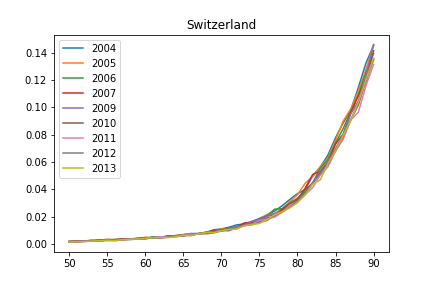
\includegraphics[width=\linewidth]{images/mortality_female_9.png}
\endminipage\hfill
\caption{Probability of dying from age $x$ to $x+1$ in 9 different years by country. \textit{Source:} Human Mortality Database}
\label{dying_female}
\end{figure}



\begin{figure}[H]
\centering \textbf{Male population}\par\medskip
\minipage{0.32\textwidth}
  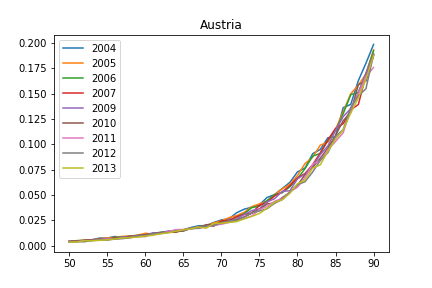
\includegraphics[width=\linewidth]{images/mortality_male_1.png}
\endminipage\hfill
\minipage{0.32\textwidth}
  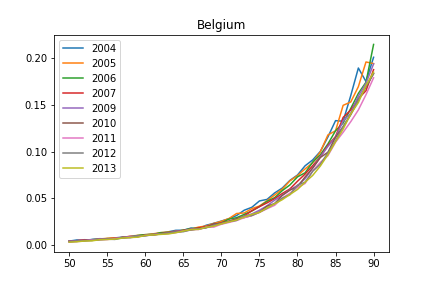
\includegraphics[width=\linewidth]{images/mortality_male_2.png}
\endminipage\hfill
\minipage{0.32\textwidth}%
  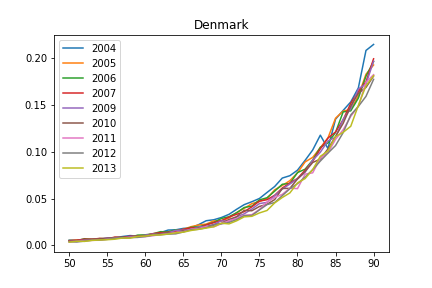
\includegraphics[width=\linewidth]{images/mortality_male_3.png}
\endminipage \hfill
\minipage{0.32\textwidth}
  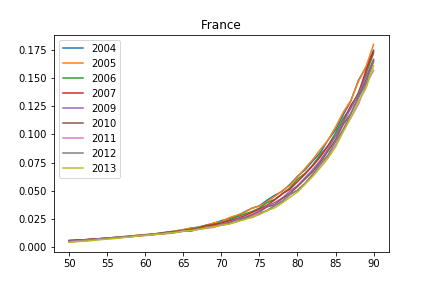
\includegraphics[width=\linewidth]{images/mortality_male_4.png}
\endminipage\hfill
\minipage{0.32\textwidth}
  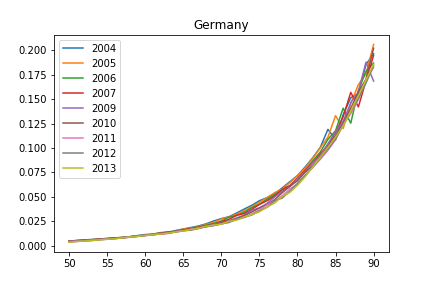
\includegraphics[width=\linewidth]{images/mortality_male_5.png}
\endminipage\hfill
\minipage{0.32\textwidth}%
  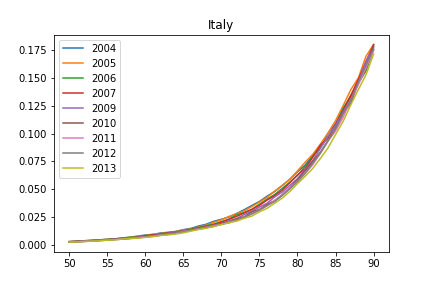
\includegraphics[width=\linewidth]{images/mortality_male_6.png}
\endminipage\hfill
\minipage{0.32\textwidth}
  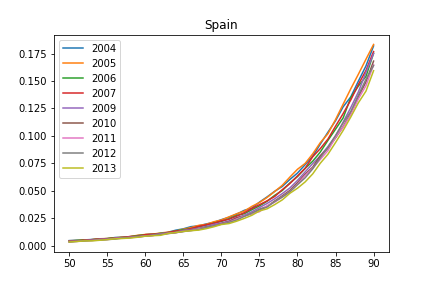
\includegraphics[width=\linewidth]{images/mortality_male_7.png}
\endminipage\hfill
\minipage{0.32\textwidth}
  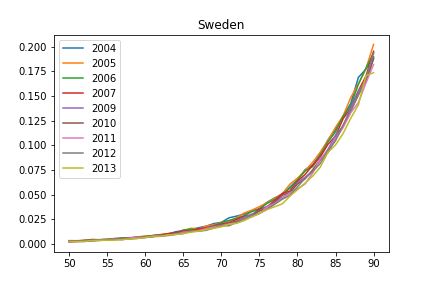
\includegraphics[width=\linewidth]{images/mortality_male_8.png}
\endminipage\hfill
\minipage{0.32\textwidth}%
  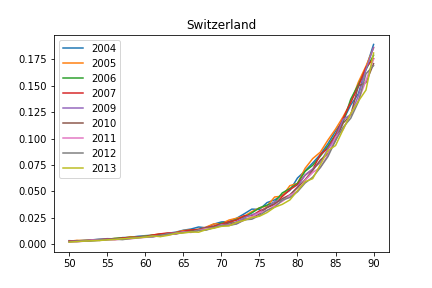
\includegraphics[width=\linewidth]{images/mortality_male_9.png}
\endminipage\hfill
\label{dying_male}
\caption{Probability of dying from age $x$ to $x+1$ in 9 different years by country. \textit{Source:} Human Mortality Database}
\end{figure}



Given the little variation over time, as third step, we compute an average of the mortality risk for all ages and countries.
For instance, the probability of dying from age 50 to age 51 in Austria will be computed by summing up all the death risk at age 50 and then dividing by the number of years considered. Figure \ref{fig:averages} represents these averaged probability for the female and male population, respectively. \\



\begin{figure}[H]
    \centering \textbf{Average risk by country}\par\medskip
    \begin{minipage}{.5\textwidth}
        \centering
        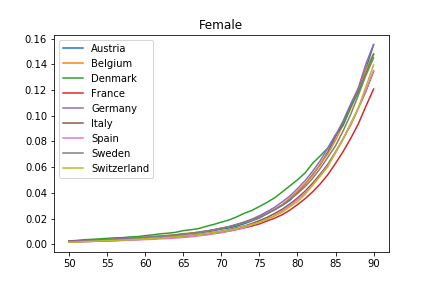
\includegraphics[scale=.5]{images/Average_mortality_female.png}
    \end{minipage}%
   \begin{minipage}{.5\textwidth}
        \centering
       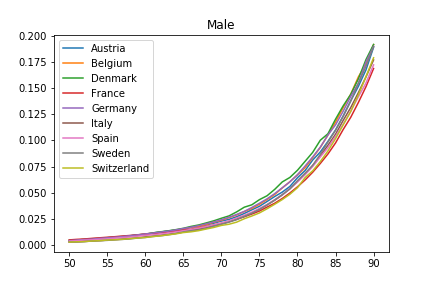
\includegraphics[scale=.5]{images/Average_mortality_male.png}
    \end{minipage}
    \caption{Average probability of dying from age $x$ to $x+1$   over 9 years by country. \textit{Source:} Human Mortality Database }
    \label{fig:averages}
\end{figure}

As fourth step, we computed an average over all countries to obtain a \lq\lq single'' mortality regime.   

\begin{figure}[H]
    \centering \textbf{Average risk}\par\medskip
        \centering
        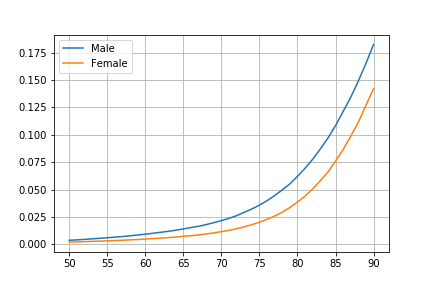
\includegraphics[scale=.5]{images/Average_mortality_all_countries.png}
    \caption{Average probability of dying from age $x$ to $x+1$   over 9 years, all countries. \textit{Source:} Human Mortality Database }
    \label{fig:averages}
\end{figure}

Clearly, this mortality regime is a synthetic measure that aggregates data from different countries, and, as such, it is inevitably introducing some bias. However, given that these European countries reasonably share some similarities, we opted for this strategy rather than estimating mortality for each country separately. The reason is that if we were to follow strategy (2), we would have ended up with estimates...
A second remark is that respondents in SHARE were also interviewed in the year 2015. However, the HMD provides information on mortality data up to 2013 for some countries (e.g. Austria, Italy, and Spain).\\
Since we wanted to compute an average of the mortality risk by age over the selected countries, we did not want to count the extra observation for the countries which had data up to 2015 and therefore we decided to exclude 2015. Again, this will introduce some inaccuracy, as we are comparing the mortality regime of two slightly different time horizons (from 2004 to 2013 in the case of HMD and from 2004 to 2015 for SHARE data). 










\end{document}